%
% Classical Networking Protocols
%

\dropcap{T}{o} set the context for our upcoming treatment of quantum networks, we begin by discussing \textit{classical} networks, and some of the key protocols behind their operation.

\section{Classical networking protocols} \label{sec:classical_nets} \index{Classical networking protocols}

\dropcap{T}{here} have been numerous approaches employed in the past for sharing communications links between multiple users\index{Shared communication channels}. This includes:
\begin{itemize}
	\item Channel-switching: an entire communications channel is designated for exclusive use by a given user. \index{Channel-switched networks}
	\item Packet-switching: data is divided into packets, which are routed independently by the network, being reconstructed by the recipient once all packets have been received.\index{Packet!Switching}
	\item Time- or frequency-multiplexing: each user is designated a particular frequency spectrum or series of time-slots exclusively for their use. \index{Time-multiplexing}\index{Frequency-multiplexing}
	\item Code Division Multiple Access (CDMA): all users can broadcast over a channel simultaneously, and the construction of the coding technique enables demultiplexing of the distinct signals, despite their interference with one another.\index{Code Division Multiple Access (CDMA)}
	\item Ethernet: all users are free to broadcast\index{Broadcast networks} over a shared channel at will, and \textit{collision detection}\index{Collisions!Detection} identifies when packets interfere, after which they are discarded and rebroadcast following a random waiting period, repeating until success.\index{Ethernet}
\end{itemize}

Nowadays packet-switched networks have become the norm in most digital networks, as they facilitate far greater efficiency in the use of network bandwidth, and are more easily scaled to greater numbers of users in a dynamic and ad hoc manner. It is foreseeable the same trend will continue with quantum technologies, especially given their initial high cost, where maximising network utility is paramount.

In this work we will focus on packet-switched networks when we later introduce our quantum networking protocols. However, with sufficient flexibility in the design of our upcoming quantum protocols, packet-switched networks can easily be made to effectively implement channel-switched, or time-/frequency-multiplexed communication.

%
% TCP/IP
%

\subsection{TCP/IP} \index{Transmission Control Protocol/Internet Protocol (TCP/IP)}

The present-day internet is built on top of a protocol stack comprising primarily the Internet Protocol (IP), User Datagram Protocol (UDP), and Transmission Control Protocol (TCP). Most commonly, these are simply referred to as TCP/IP. These define a stack of different layers of abstraction for communicating data packets between nodes in a network, determining their routing, and enforcing any quality of service requirements.

%
% Internet Protocol
%

\subsubsection{Internet Protocol} \index{Internet Protocol (IP)}

IP is the standard protocol employed in the internet for P2P communication of data packets. It is a low-level protocol that encapsulates digital data into packets containing a header field, which specifies routing information, most notably the IP addresses of the source and destination. IP does not enforce any kind of quality control, which is instead delegated to higher-level protocols like TCP (Sec.~\ref{sec:TCP}), a higher-level of abstraction built on top of IP (Sec.~\ref{sec:TCP}).

Multiple packets with the same source and destination needn't follow the same route -- the routing is determined dynamically in realtime by routers, based on network characteristics such as load or latency. Thus, packets belonging to the same underlying data may arrive out of order, or some may go missing altogether. IP does not address these issues, instead engaging in only `best-effort' delivery. 

In IP there is no central authority with knowledge of the state of the entire network, which tells routers in the network how to best route packets. Thus, IP must be complemented with up-to-date routing tables, held by routers/nodes in the network, which make routing decisions on a per-packet basis. This is achieved using gateway protocols, discussed next.

%
% User Datagram Protocol
%

\subsubsection{User Datagram Protocol} \index{User Datagram Protocol (UDP)}

The UDP is a simple protocol built on top of IP, based on a `send-and-forget' principle for sending data packets. That is, there is no quality of service guarantee, and no notifications are provided to the sender as to whether packets successfully reached their destination. However, a checksum (hash) forms a part of the packet headers to enable error detection by the recipient. The lack of quality control bypasses the associated latency, making it particularly useful in time-critical applications, where the late arrival of a packet is useless and therefore needn't be retransmitted.

UDP is connectionless, meaning that no designated connection is established between hosts. Instead data is simply transmitted and then forgotten about. The receiver may not even be operational on the network, in which case the packets are lost without notice.

Key examples for the use of UDP are realtime audio and video transmission. If a packet associated with a frame in a video link is delayed and arrives several frames late, it is useless, since it is associated strictly with a previous frame in the video that has already passed. Quality control, in the form of contacting the sender to request a retransmission, would therefore achieve nothing. This applies similarly to live audio streaming, such as voice over IP (VoIP)\index{Voice over IP (VoIP)}, where the late arrival of a packet cannot possibly be correctly inserted into the audio playback and might as well be discarded.

Therefore, UDP prioritises latency over reliability, and is best suited to time-critical applications where quality of service is not relevant.

%
% Transmission Control Protocol (TCP)
%

\subsubsection{Transmission Control Protocol} \label{sec:TCP} \index{Transmission Control Protocol/Internet Protocol (TCP/IP)}

TCP differs from UDP in that it intrinsically supports quality control. The protocol is able to determine whether a packet successfully reached its destination, and if not, retransmit it as often as necessary to guarantee packet delivery. A checksum is also included in packet headers to enable error detection. This quality control has made TCP the dominant protocol employed in the present-day internet, where, in most scenarios, we wish to guarantee that data has been correctly delivered -- if an email is missing random segments of its text, users will become irate very quickly!

TCP is connection-oriented, meaning that a handshaking protocol establishes a dedicated bidirectional channel between two hosts. It also enforces packet reordering, to counter out-of-order packet arrival.

However, the enforced quality control and handshaking protocols incur a network performance overhead that UDP does not, since handshaking protocols consume bandwidth. Thus, TCP should not be used instead of UDP if there are no quality of service requirements.

%
% Ethernet
%

\subsection{Ethernet} \index{Ethernet}

Ethernet is a networking protocol based on `broadcasting' on a shared network. This model is particularly suited to local area networks (LANs), where all users share a single communications channel rather than dedicated P2P links, as shown in Fig.~\ref{fig:ethernet}.

\begin{figure}[!htbp]
	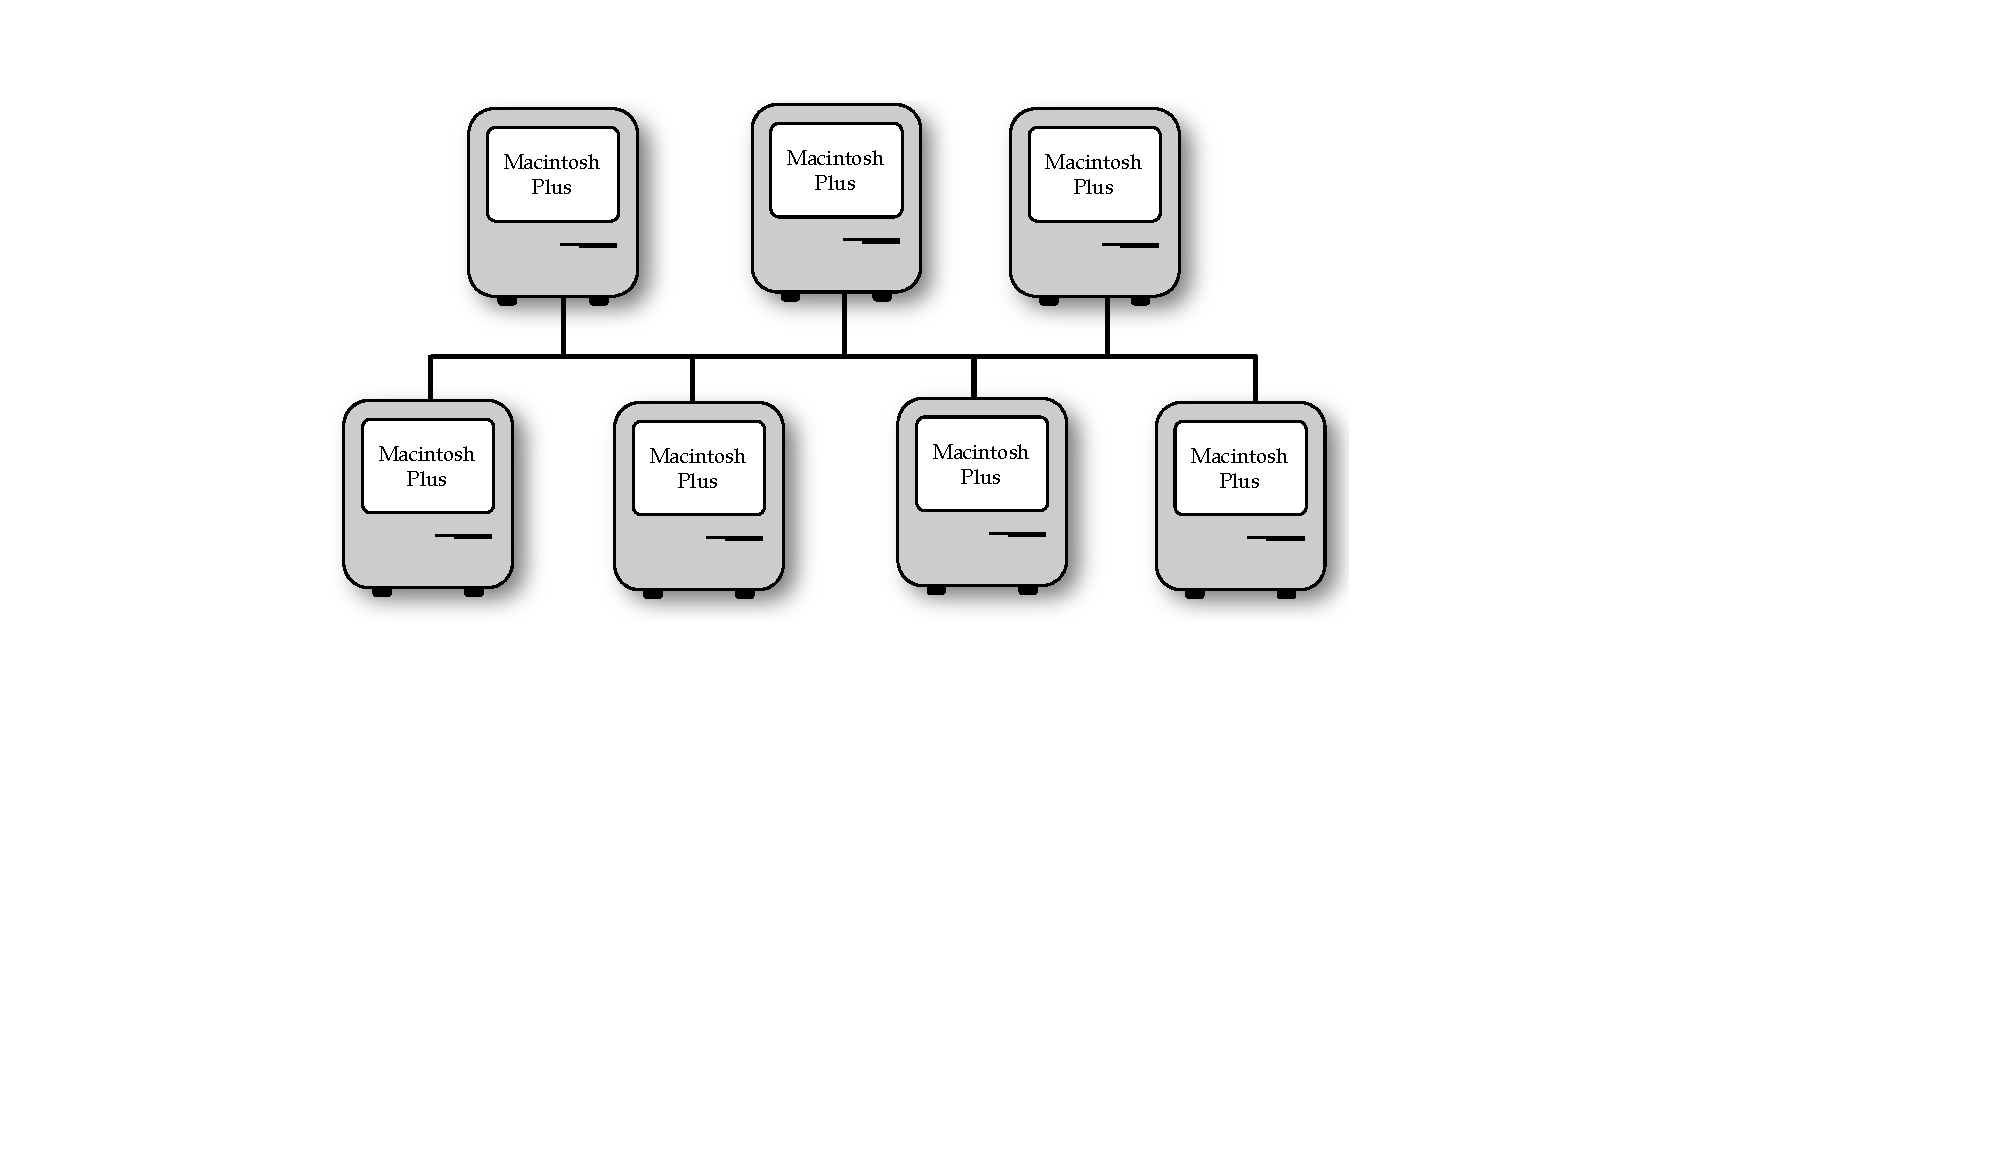
\includegraphics[clip=true, width=0.475\textwidth]{ethernet}
	\captionspacefig \caption{The topology of an Ethernet network, whereby all users share a common channel, which they can broadcast to at their leisure. If data packets collide, it is detected via the packets' checksums, and the corrupted packets may be re-broadcast after a random `backoff' waiting period, repeating this process until packet delivery is successful. Obviously the chance of collisions occurring increases with the number of connected users, thus network performance is inversely related to the number of nodes.} \label{fig:ethernet}
\end{figure}

In the Ethernet protocol, every user is free to broadcast data onto the shared channel as they please -- all users transmit to, and receive from a single shared channel. However, clearly sometimes packet `collisions' will occur\index{Collisions!Handling}, resulting in packet corruption. To overcome this, Ethernet packets contain a checksum that can be used to verify upon arrival whether a packet has been corrupted by a collision. If a collision is detected, the respective users are able to re-broadcast, following a randomly chosen waiting period (known as `backoff')\index{Backoff}. Collisions therefore reduce network performance, and it follows that network bandwidth decreases with the number of users competing for bandwidth\footnote{Think of that awkward dinner table conversation, where two people start talking simultaneously (Peter \& Jon). It's immediately obvious to them both that they are interfering with one another, and if they were to just talk over one another (packet collision), no one would understand either of them. So, they both awkwardly pause, before starting to speak again. In a \textit{really} awkward conversation, they will both start again simultaneously, after which there will be an even longer awkward pause before recommencing. Eventually, this self-regulating system will resolve itself probabilistically, with a sole victor controlling the airwaves, commanding the attention of the listeners. Provided that all dinner guests adhere to social etiquette and backoff appropriately, with repeated conversations, all guests will statistically receive an equitable share of attention, albeit with some wastage of conversation time owing to the periods of silence. Clearly, the proportion of the time wasted due to collisions will scale up with the number of guests, limiting the protocol to not-too-large tables (or very quiet guests).}.

From this protocol, any given packet will eventually be successfully transmitted uncorrupted, collision-free, albeit with uncertain timing that grows with the number of competing users. For this reason, the Ethernet protocol is not ideal for time-critical applications requiring hard guarantees on network latency.

The beauty of this approach is that only a single channel is required for connecting all users. No dedicated P2P connections are required. As the number of users increases, the complexity of the network topology does not -- requiring only the addition of a node to the existing backbone. For small LANs this is clearly reasonably functional. However, as the size of networks increases, the rate at which packet collisions occur increases, resulting in a reduction in network bandwidth. Thus, the Ethernet protocol is ideally suited to small LANs, but is clearly not viable at a global level, where network competition is astronomical and the overhead from backoff would reduce network performance to a standstill, wasting most of the bandwidth.

Another elegant feature of the Ethernet protocol is that bandwidth allocation is self-regulating, with bandwidth fairly and equitably allocated between users, not prioritising any user over another. This applies even in completely ad hoc networks, with users joining and leaving the network willy nilly. Provided all users are correctly and honestly implementing the \textsc{Broadcast and Backoff} protocol, network bandwidth is allocated evenly amongst users, and no mediating, overriding central authority is needed to oversee network resource allocation. This allows Ethernet networks to be truly `plug-and-play'.

%
% Gateway Protocols & Routing Tables
%

\subsection{Gateway protocols \& routing tables} \label{sec:gateway} \index{Gateway protocols} \index{Routing!Tables}

In the absence of a central mediating authority, routing decisions must be made by individual nodes in the network, upon receipt of packets. For routers to make sensible routing decisions, they must have some idea of the overall structure and state of the network. This is achieved using gateway protocols, which communicate information about the state of the network on a nearest-neighbour basis. There are various gateway protocols in use, with the Exterior Gateway Protocol (EGP)\index{Exterior Gateway Protocol (EGP)} and Border Gateway Protocol (BGP)\index{Border Gateway Protocol (BGP)} being very common.

We let every node in the network have a routing table, initially empty, that will ultimately be populated with information on how to best route incoming packets further along the route to their destination.

To mitigate the need for a central authority, nodes engage in only nearest neighbour communication, sharing their routing tables with one another, to query about the distance metrics (Sec.~\ref{sec:costs}) associated with routes to different destinations. This communication is taking place regularly, and as nodes' routing tables become populated, updating in real-time, they will (hopefully) reach a steady-state. From these tables, single-source shortest path algorithms (Sec.~\ref{sec:single_source_sp}) can be applied by nodes to construct a complete picture of costs to every point in the network. Such a nearest neighbour algorithm is effectively a distributed breadth-first-search\index{Breadth-first-search (BFS) algorithm} algorithm (Sec.~\ref{sec:path_exp}).

%
% Network Hierarchies
%

\subsection{Network hierarchies} \index{Network!Hierarchies}

The disadvantage of Ethernet's \textsc{Broadcast and Backoff} principle is that packets are often wasted -- whenever a collision occurs. Because there is no mediating central authority, packet collisions are a certainty in a heavily-utilised shared network, each time resulting in packet loss, and an associated reduction in usable network bandwidth.

To the other extreme, we could have dedicated P2P channels between every pair of users. Then there would be guaranteed no packet collisions, and therefore maximum bandwidth efficiency, but the network would be extremely costly, and plug-and-play extremely challenging.

To address this dilemma, the topology and subdivision of networks need to be carefully designed. If we consider a large organisation, for example, potentially networking thousands of desktop PCs, the bandwidth wastage associated with packet collisions could grind the entire network to a halt, were all thousands of PCs to be communicating large amounts of data simultaneously. However, if a hierarchy of subnetworks could be implemented, rather than a single monolithic network, efficiency could be improved drastically.

Suppose our hypothetical organisation had several different departments, and users had a tendency to communicate primarily with other users in the same department. By defining distinct departmental subnets, which individually implement Ethernet, but interconnect with one another using an alternate routing framework, we can easily see that many unnecessary packet collisions may be entirely avoided. That is, why broadcast data to users who we know don't want it? A simple example of this is shown in Fig.~\ref{fig:net_hierarchy}.

\begin{figure}[!htbp]
	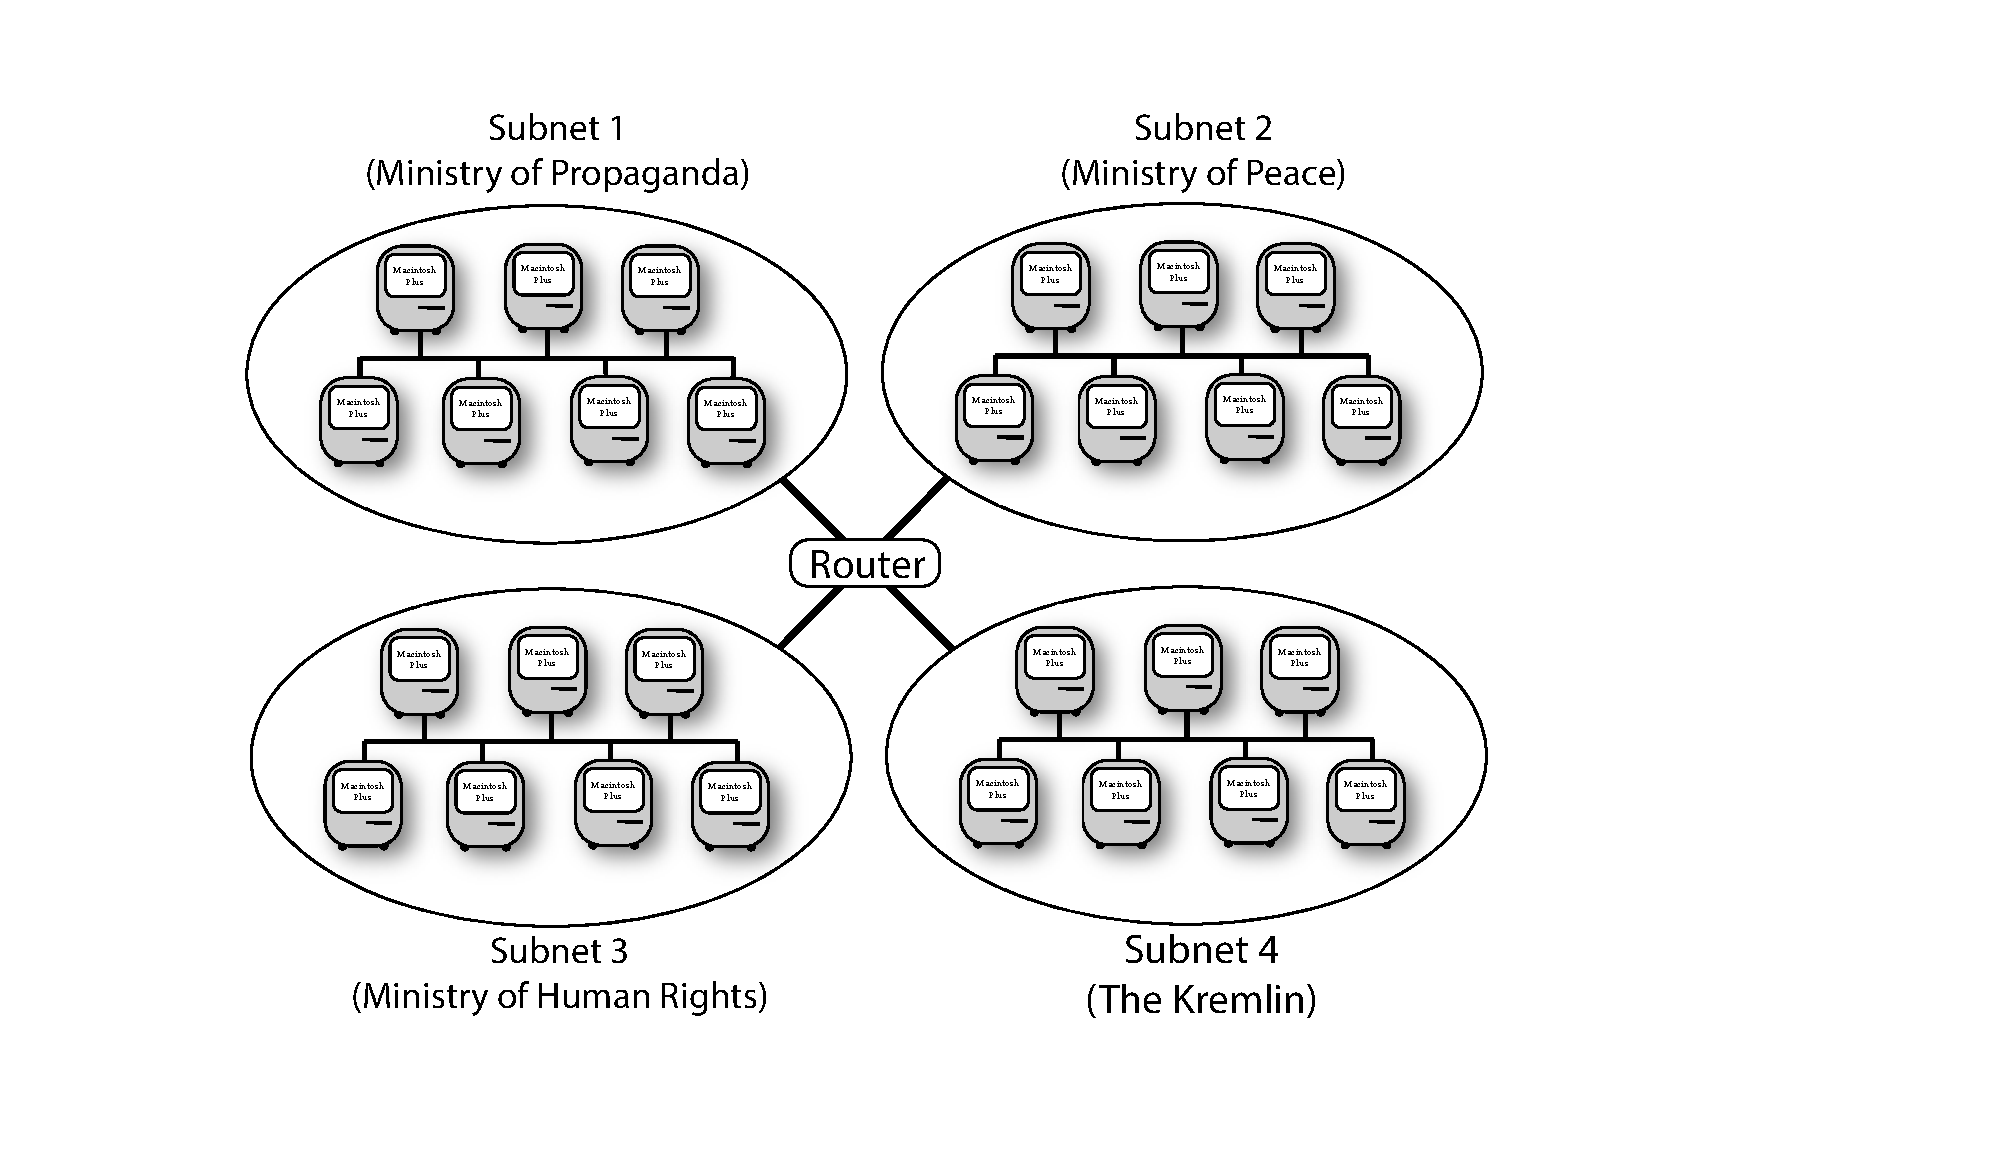
\includegraphics[clip=true, width=0.475\textwidth]{network_hierarchy}
	\captionspacefig \caption{Simple example of a network with two levels in its hierarchy. At the lowest level are 4 different subnets belonging to different departments within an organisation, each of which implements Ethernet networking. Above this, the subnets connect together in a star network via a central router. By subdividing the network hierarchy as such, if most traffic emanating within a subnet stays within that same subnet, collisions between packets on different subnets are avoided, thereby improving the efficiency of the subnets' Ethernet implementations.} \label{fig:net_hierarchy}
\end{figure}

Extending upon this simple intuitive example, enormous amounts of research and development have been invested into the design of network hierarchies, and how to optimise their efficiency. A pressing consideration in the design of network protocol stacks is therefore to accommodate for multiple routing protocols, and enabling their inter-compatibility.